\chapter{Experimental Results}
\label{chapter:experiments}

MOD* Lite is a domain independent algorithm and can be applied to any virtual environment with given $n$ objectives. These objectives could be whether \textit{maximized} or \textit{minimized}. The vital assumption about objectives is their independence from each other. If two objectives could effect each other in a positive or negative manner, this might reduce or expand objectives vector size, which is out of this work's scope. Thus, we assume that each defined objective is considered in different perspective and can not be transferred to each other.

The algorithm is tested on various environments with different scenarios. However, as it is not possible to exemplify all possible cases, specific and several extreme conditions are selected for experiments. MOD* Lite is compared with MOA* that guarantees optimal solutions in fully observable multi objective environments and MOGPP, a classic genetic solution which can be used for finding paths with multi objective cases.

For testing, all algorithms are implemented in Java language and run under Linux environment which has Intel Core2 Quad CPU running at 2.33GHz and 4 GB of RAM.

All tests are done on 2-D grid maps as detailed in Subsection \ref{envProperties}. In these tests, the agent tries to find available non-dominated best paths with respect to two objectives, path length and risk taken from threat zones. Thus, the agent endeavours to minimize both objectives and tries to find \textit{shortest} and \textit{safest} paths.

For all test cases, several parameters of MOGPP algorithm must be tuned. For instance; number of elitist individuals are $5$, population count and maximum iteration are $50$, and cross-over and mutation ratios are taken as $0.8$ and $0.05$, respectively. As MOGPP constructs initial paths randomly, each execution of the algorithm might not give exactly same results at the same execution time even the maps are equal. Thus, all given execution times and selected paths are considered as the average of 10 different executions for MOGPP.

\section{Fully Observable Tests}

First of all, it must be shown that MOD* Lite is complete and gives optimal and/or sub-optimal results in fully observable environments. The performance comparison is done in two dimensions, execution times and paths they generate (path quality), respectively.

In the first set of tests, randomly generated fully observable maps with different sizes (25 x 25, 50 x 50, 75 x 75, 100 x 100, 125 x 125 and 150 x 150), are used. Each of these maps have nearly 30\%-32\% percent threat zone and 14\%-16\% percent obstacle ratio. Agent's initial and target locations are also taken randomly. For this case, execution times and generated paths' costs for different sized maps are given in Figure \ref{fig:rand_fully} and Table \ref{table:randPaths}. As seen from path qualities, MOA* finds optimal results and MOD* Lite finds optimal and/or sub-optimal results while gradually increases on the computation time manner. Although MOGPP works on similar times with MOA*
 especially for large scaled maps, it fails to find optimal or sub-optimal paths. One could set maximum iteration and population count to larger numbers to converge path quality to optimality, but this case increases execution time exponentially. Thus, more modest parameters are chosen for MOGPP to enforce the algorithm to yield reasonable results within expected time. 
 
Notice that taken risk values depend on environmental properties and should not be compared between different sized maps.

\begin{figure}
\centering
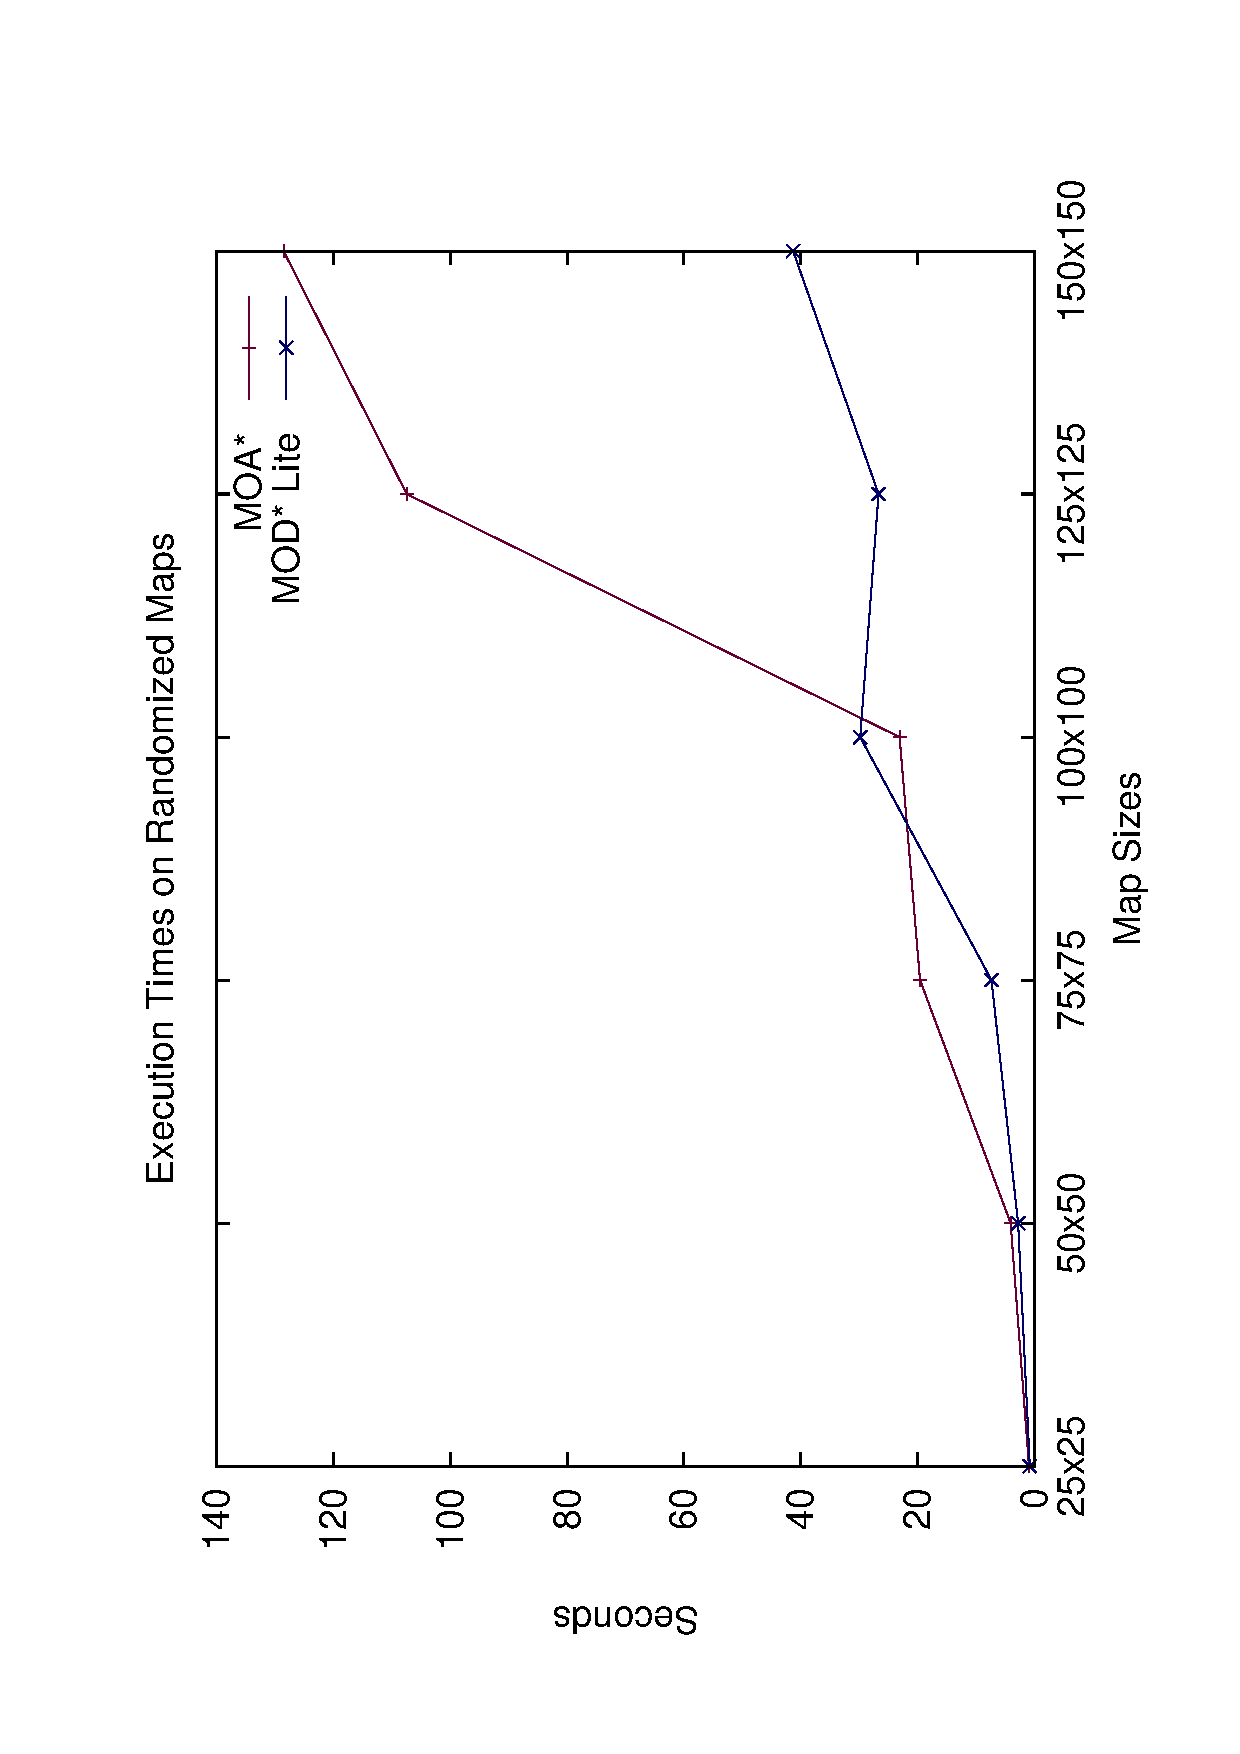
\includegraphics[width=4in, angle=270]{experimental/w_mogpp/randomized}
\caption{Execution Times of Randomly Generated Fully Observable Maps}
\label{fig:rand_fully}
\end{figure}

\begin{table}[ht]
	\caption{Non-dominated Path Costs For Randomized Maps} % title of Table
	\centering
    \begin{tabular}{l l l l}
        \hline
        Map Size  &  MOD* Lite  &  MOA*  &  MOGPP \\ [0.5ex] \hline
        25 x 25   &  (49, 571)  &  (49, 571)  &  (49, 3523)
		   \cr    &  (51, 10)   &  (51, 10) &  (51, 764) 
		   \cr	 &			   &				&  (53, 58)\\ 
        50 x 50   & (99, 982)   & (99, 982)  &  (103, 7399)
		   \cr	  &	(101, 0)   &  (101, 0)  &  (121, 178)
		   \cr	 &			   &				&  (123, 0)\\
        75 x 75   & (149, 1549) & (149, 115) & (175, 730)
		   \cr	  &  (151, 221) & (153, 0) & (187, 272)
		   \cr	  &  (153, 0)	&			& (201, 0)\\
        100 x 100 & (199, 10) & (199, 10) & (301, 2357)
		   \cr    & (201, 4) & (201, 4) & (329, 1087)
		   \cr    & (203, 0) & (203, 0) & (349, 746)\\ 
        125 x 125 & (90, 1036) & (90, 1036) & (225, 10677)
		   \cr	  & (92, 293) & (92, 293) & (239, 2249)
		   \cr	  & (94, 165) & (94, 165) &
		   \cr	  & (96, 101) & (96, 101) &				\\
        150 x 150 & (126, 128) & (126, 128) & (191, 14720)
		   \cr	 &			   &				&  (207, 5316)        
    		   \cr	 &			   &				&  (211, 312) \\ [1ex]
        \hline
    \end{tabular}
	\label{table:randPaths}
\end{table}

In the second set of tests, each algorithm is executed on handcrafted maps with same sizes, threat zone and obstacle ratio with randomized tests as indicated in previous test case. These maps are also assumed fully observable and agent's initial and target locations are taken randomly. All handcrafted test environments \textit{guarantee} that at least two non-dominated paths will be available. Execution times are shown in Figure \ref{fig:hand_fully} and generated paths' costs are given in Table \ref{table:handPaths}.

\begin{figure}
\centering
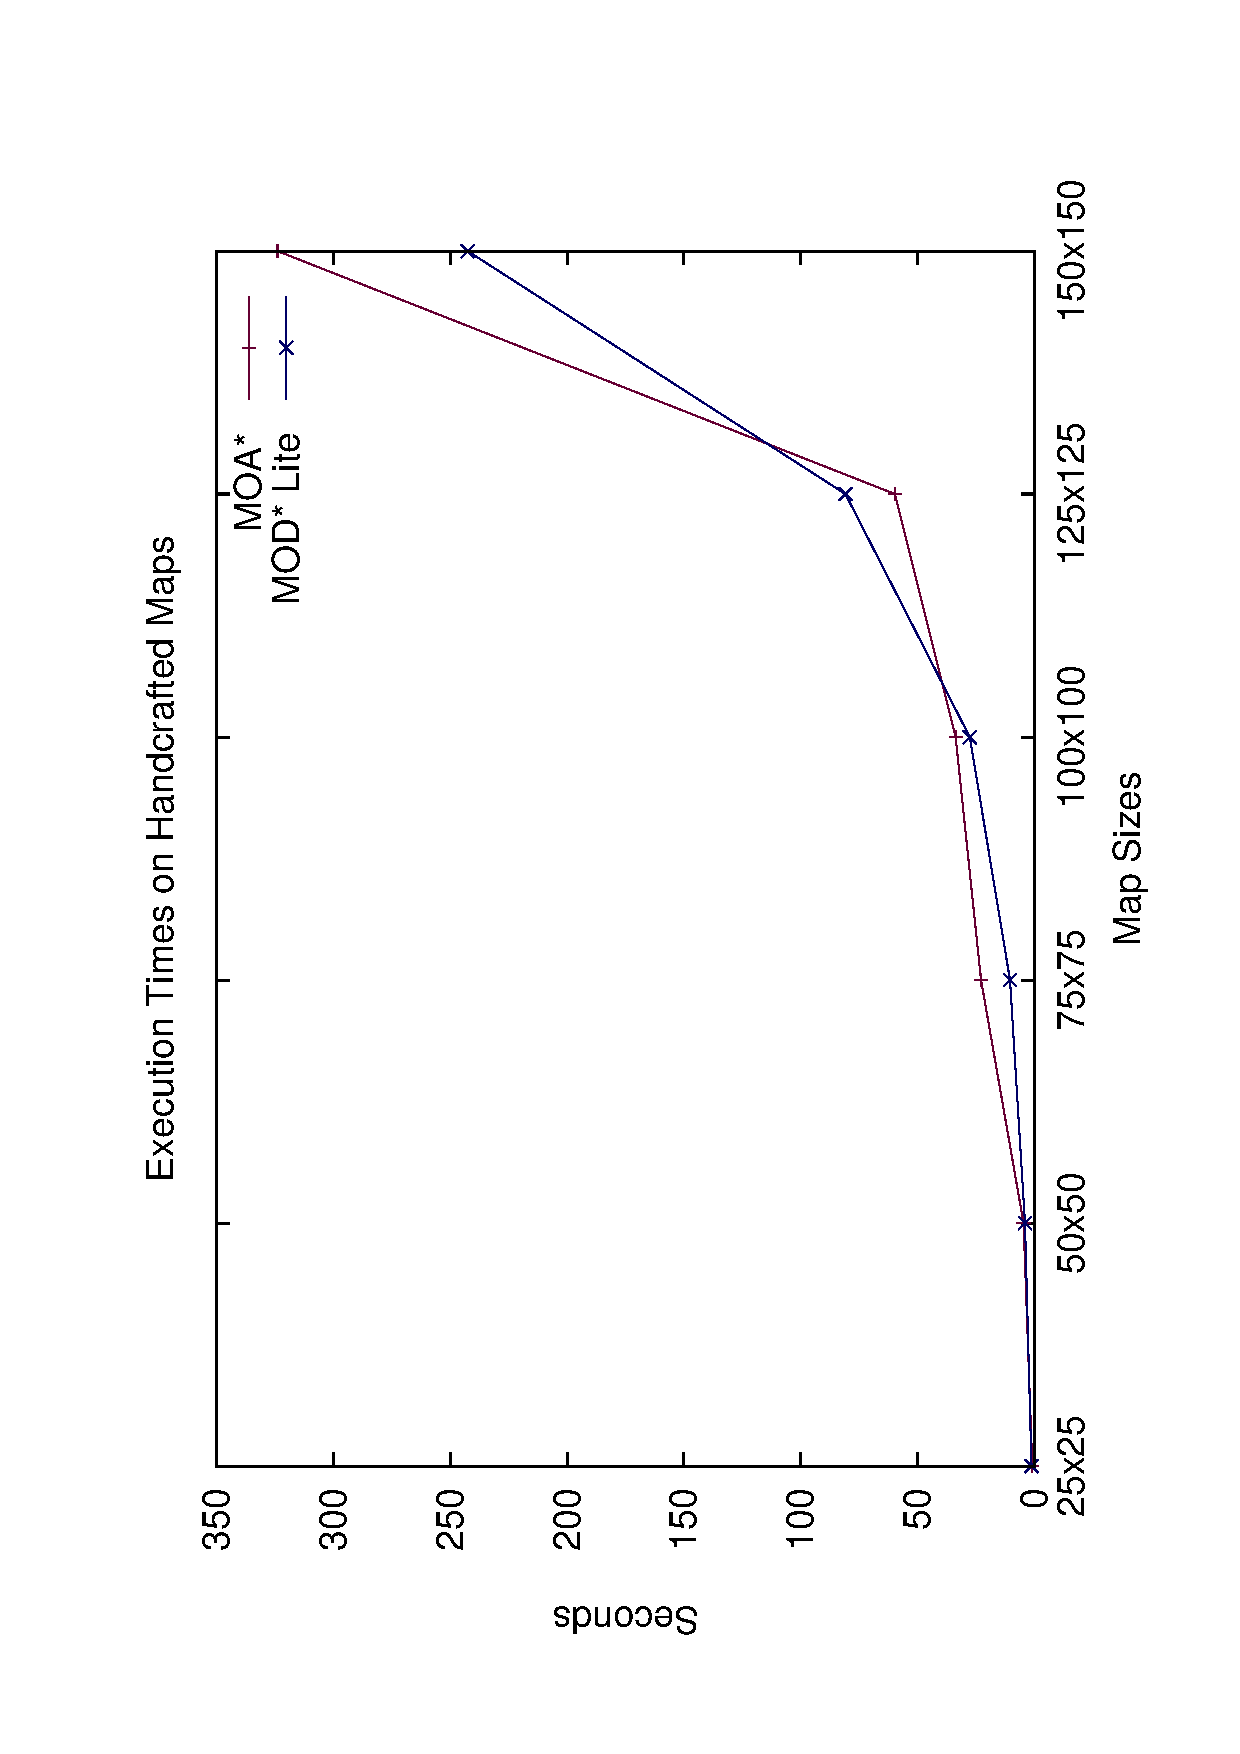
\includegraphics[width=4in, angle=270]{experimental/w_mogpp/handcrafted}
\caption{Execution Times of Handcrafted Fully Observable Maps}
\label{fig:hand_fully}
\end{figure}

\begin{table}[ht]
	\caption{Non-dominated Path Costs For Handcrafted Maps}
	\centering
    \begin{tabular}{l l l l}
        \hline
        Map Size  &  MOD* Lite  &  MOA*  &  MOGPP\\ [0.5ex] \hline
        25 x 25   &  (49, 722)  &  (49, 722)  &  (53, 1227)
		   \cr    &  (51, 505)   &  (51, 505)  &  (56, 938)
   		   \cr    &  (55, 216)   &  (55, 216)  &  (59, 216)\\ 
        50 x 50   & (99, 14)   & (99, 14)  &  (101, 1871)
		   \cr	  &	(101, 0)   &  (101, 0)  &  (125, 1156)
		   \cr	 &			   &				&  (151, 736)\\
        75 x 75   & (149, 1927) & (149, 1927) &  (235, 737)
		   \cr	  &  (151, 1329) & (151, 1329) &  (261, 372)
		   \cr	  &  (153, 279)	&	(153, 279) & (279, 0)
   		   \cr	  &  (159, 0)	&	(159, 0) & \\
        100 x 100 & (199, 1077) & (199, 144) & (297, 4390)
		   \cr	  & (201, 20) & (201, 20) & (315, 3710)
		   \cr	  & (205, 0) & (205, 0) & (395, 1861)\\
        125 x 125 & (249, 15) & (249, 15) & (391, 9516)
		   \cr    & 			 & (257, 0)  &  (445, 5358)
		   \cr	 &			   &				&  (451, 365)		   
		   \cr	 &			   &				&  (561, 0)\\
        150 x 150 & (301, 20) & (299, 145) & (266, 6110)
    		   \cr	  & 			 & (301, 20) & (270, 5915)
   		   \cr	  & 		  & (315, 0) & (284, 4530)\\ [1ex]
        \hline
    \end{tabular}
	\label{table:handPaths}
\end{table}

In execution times in Figure \ref{fig:hand_fully}, it can be seen that MOGPP increases gradually instead of an exponential growth especially on large scaled maps. However, its path quality is not good enough when compared to MOD* Lite and MOA*' s results.

There exists a remarkable point that MOA* has nearly similar results with MOD* Lite in both path quality and execution time. This case shows that even MOD* Lite is based on partially observable dynamic environments, it could also give \textit{as good results as} MOA* on stationary and fully observable environments and can be applied on those environments.

\section{Partially Observable Tests}

As discussed in previous sections; the main difference of MOD* Lite from existing classic path planning or evolutionary based algorithms is its adaptivity to partially observable dynamic environments. To show this advantage, partially observable tests are done with randomized maps of sizes 75 x 75, 100 x 100 and 125 x 125. On these maps, agent's initial and target locations are chosen to be the furthermost cells in the environment. For each map, agent' s sensor range was set between 20\% to 60\% and execution times were observed. An example search space of MOD* Lite with 30\% sensor range can be seen in Figure \ref{fig:initialSearch}. In this figure, agent is depicted with a cyan dot. The fogged gray area represents agent' s sensor range and drawn purple path through temporary goal (blue dot) can be seen.

\begin{figure}
\centering
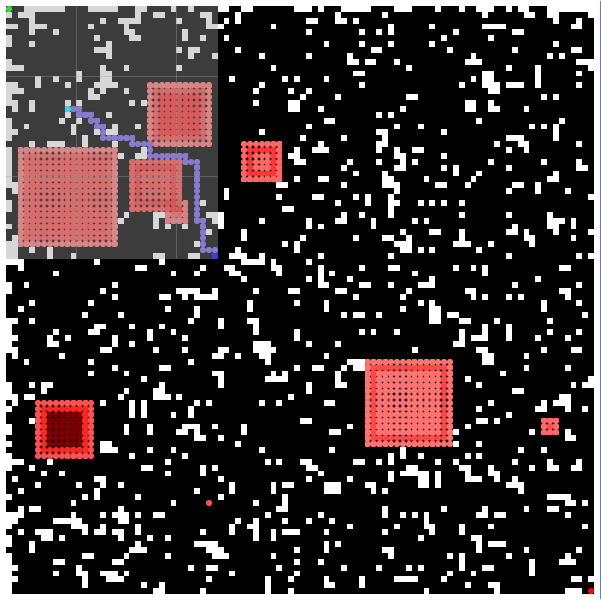
\includegraphics[width=4in]{experimental/initialSearch}
\caption{A 100x100 Partially Observable Map with 30\% Sensor Range}
\label{fig:initialSearch}
\end{figure}

In these tests, the agent starts to plan a path towards the nearest available cell within its sensor range -the temporary goal- to the actual goal with respect to Manhattan Distance. After planning, consider that agent has found three paths with costs $(15, 200)$, $(18, 230)$ and $(23, 260)$. In such cases, the agent tends to choose the path with cost $(18, 230)$, the median of paths. This ad-hoc strategy could be set explicitly according to the domain that the algorithm works on. Afterwards, it starts to follow the chosen path. When new cells are available or a weight of a cell is changed within sensor range, agent reassigns the temporary goal and re-executes the path planner algorithm. This process iterates until the agent reaches to the desired goal location.

\begin{figure}
\centering
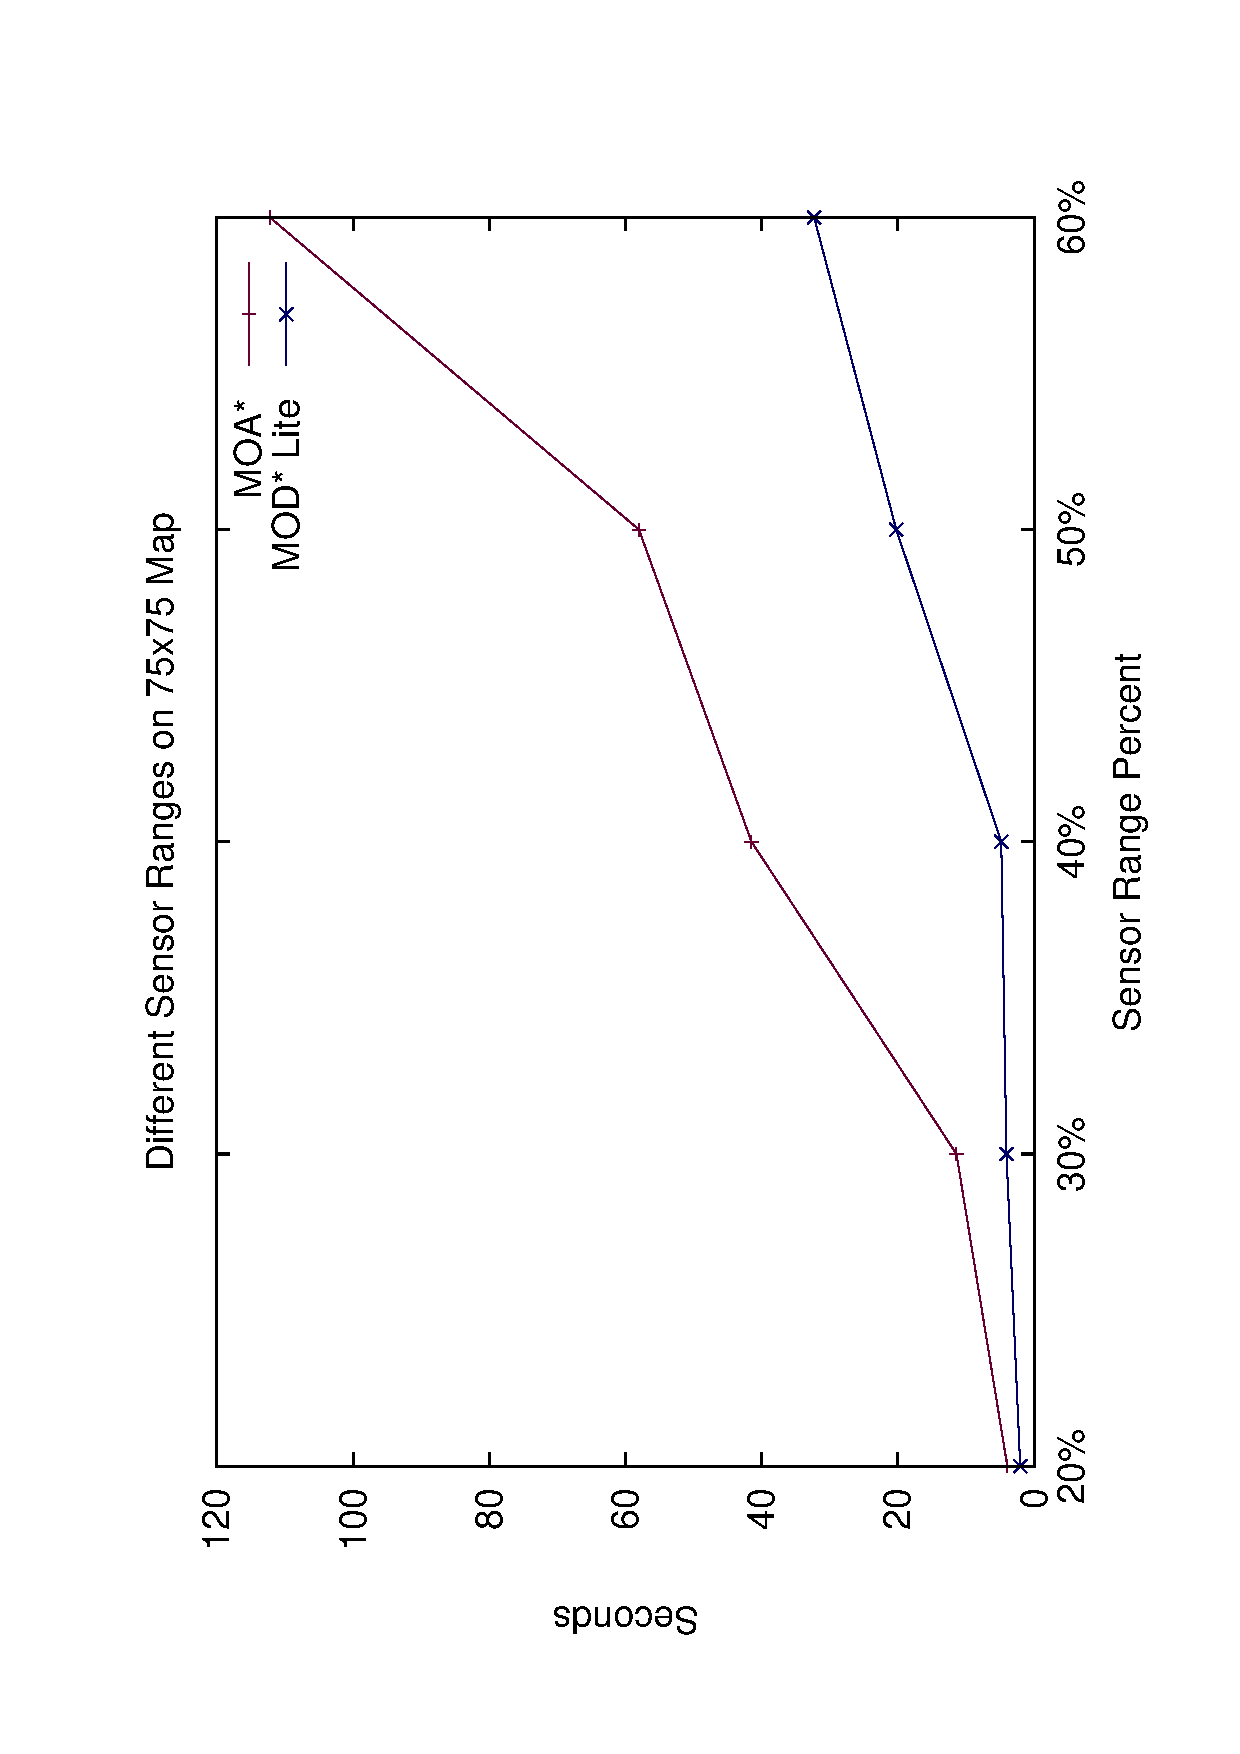
\includegraphics[width=4in, angle=270]{experimental/w_mogpp/75x75SensorRange}
\caption{75x75 Partially Observable Map on Different Sensor Ranges}
\label{fig:75x75sensor}
\end{figure}

\begin{figure}
\centering
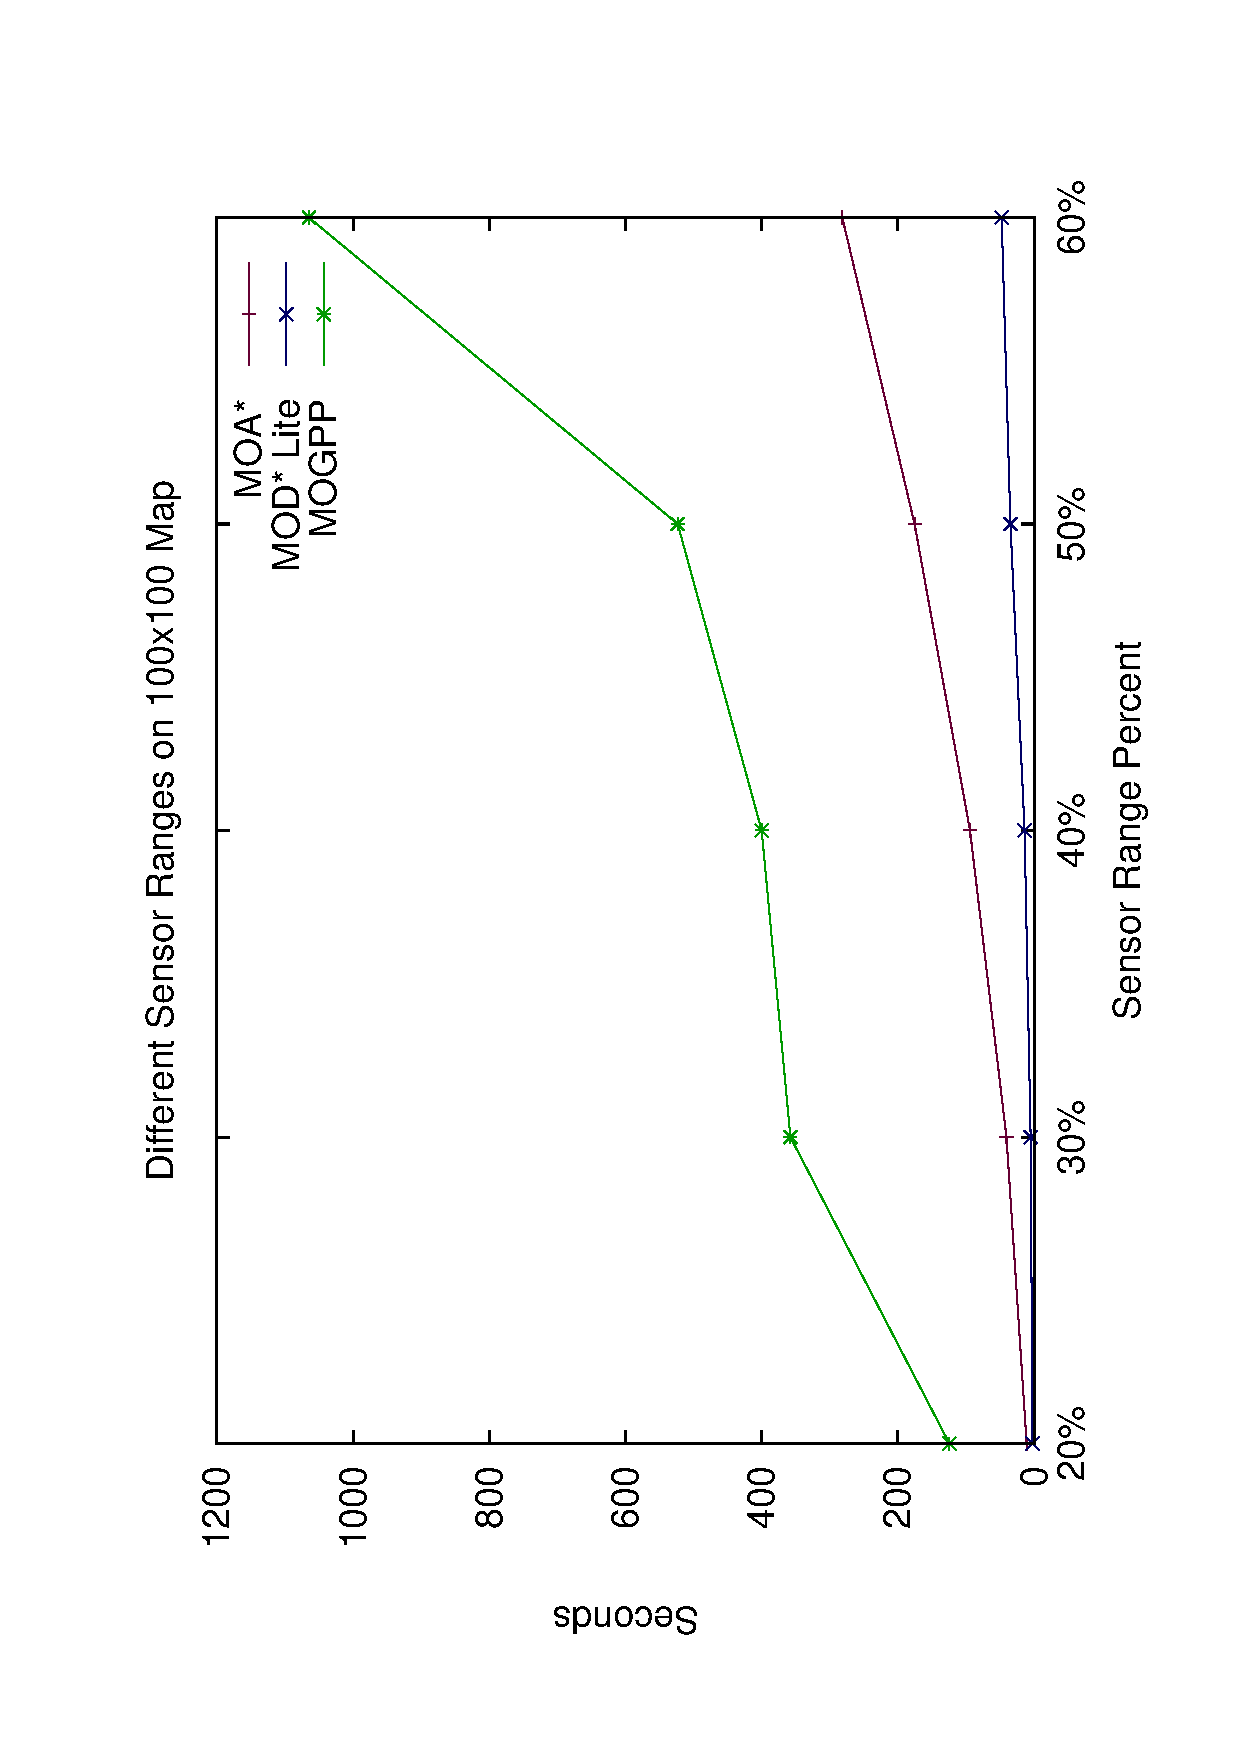
\includegraphics[width=4in, angle=270]{experimental/w_mogpp/100x100SensorRange}
\caption{100x100 Partially Observable Map on Different Sensor Ranges}
\label{fig:100x100sensor}
\end{figure}

\begin{figure}
\centering
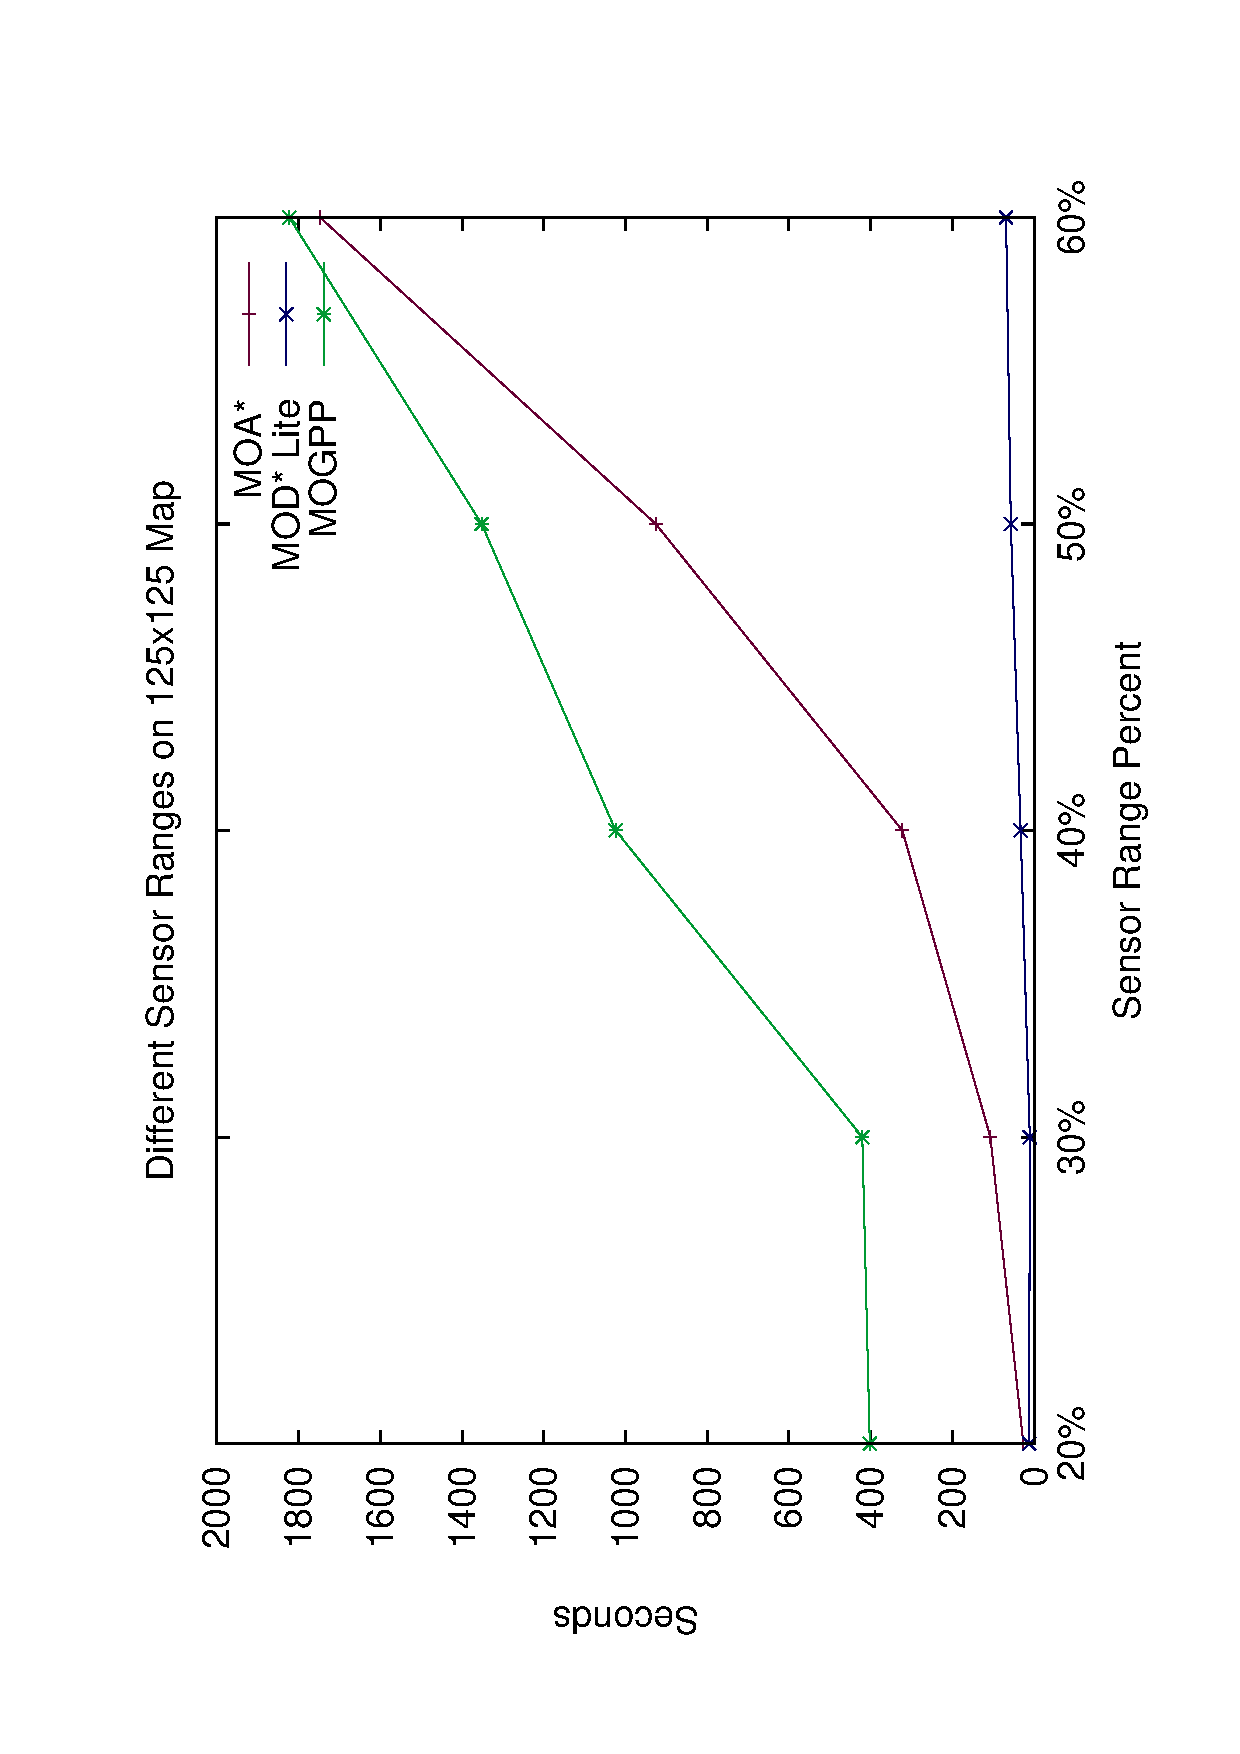
\includegraphics[width=4in, angle=270]{experimental/w_mogpp/125x125SensorRange}
\caption{125x125 Partially Observable Map on Different Sensor Ranges}
\label{fig:125x125sensor}
\end{figure}

\begin{figure}
\centering
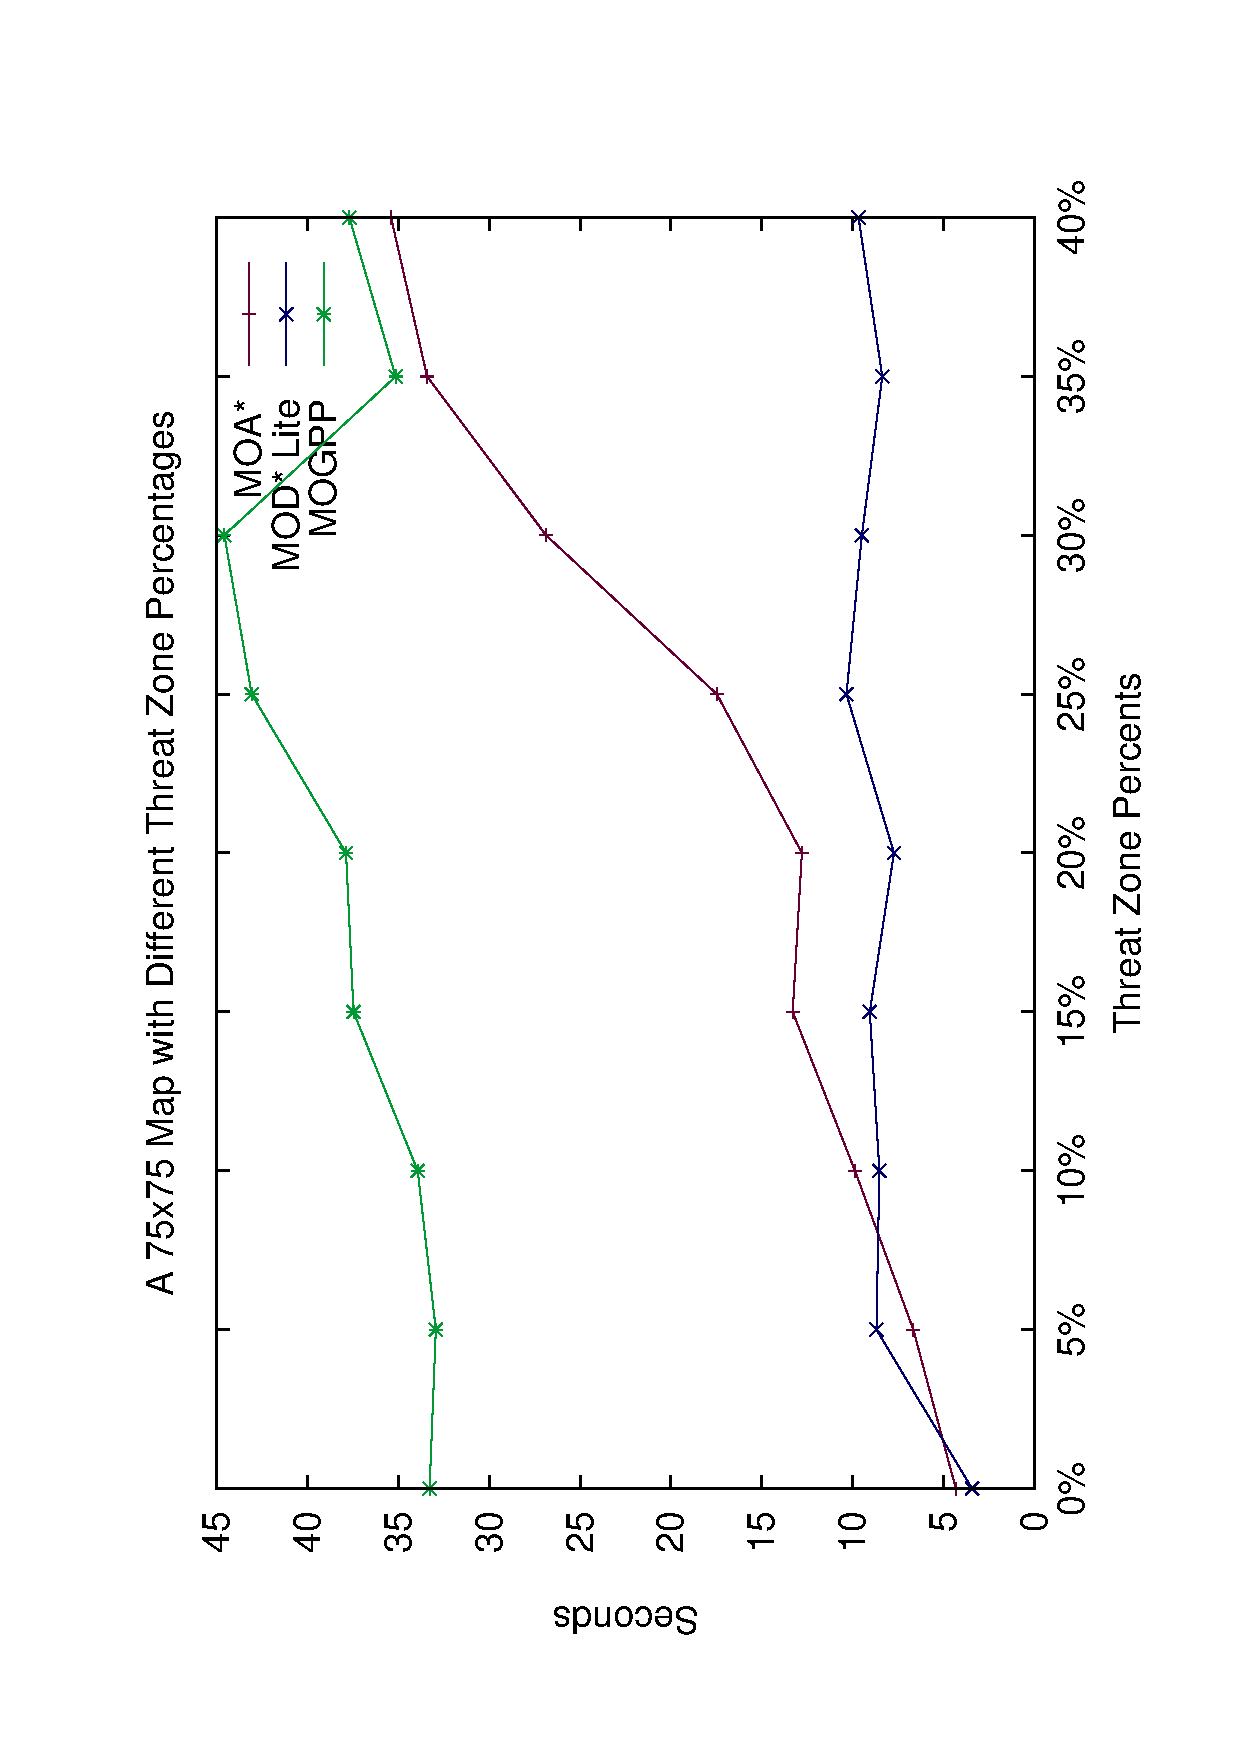
\includegraphics[width=4in, angle=270]{experimental/w_mogpp/new75x75ThreatZonePercent}
\caption{Execution times of 75x75 Fully Observable Map on Different Threat Zone Percents}
\label{fig:tzratio}
\end{figure}

%\begin{table}[ht]
%	\caption{MOGPP Execution Times on a 125x125 Partially Observable Map}
%	\centering
%    \begin{tabular}{l l}
%        \hline
%        Sensor Range	&	Execution Time (sec.)\\ [0.5ex] \hline
%        20\%			&	402.325\\
%        30\%			&	420.481\\
%		40\%			&	1024.237\\
%		50\%			&	1351.854\\
%		60\%			&	1922.415\\ [1ex]
%        \hline
%    \end{tabular}
%	\label{table:mogpp125vFrustum}
%\end{table}

The fundamental advantage of MOD* Lite can be seen very clearly on these tests. While MOD* Lite has the capability of updating only the effected states due to its incremental nature, MOA* re-plans the overall path from scratch when new parts become known and the weights of some cells have changed. This situation causes MOA* and MOGPP to work on exponentially long times. Total execution times to reach to the target for these test cases are given in Figures \ref{fig:75x75sensor}, \ref{fig:100x100sensor} and \ref{fig:125x125sensor}. As can be seen from results, MOD* Lite can easily handle the dynamical issues of the environment where MOA* and MOGPP fails. Due to discovering different parts of the environment during execution, actual traversed path's costs of MOD* Lite, MOA* and MOGPP might be slightly different from each other, where MOD* Lite could follow a better path with respect to MOA* or MOGPP or vice versa.

\section{Multi Objectivity Tests}

As threat zones and their risk values are used as the second objective, percentages of these zones also effect execution time and generated path quality. In this set of tests different threat zone percents are tested on a fully observable 75 x 75 map and results are given in Figure \ref{fig:tzratio}. It could be observed that increasing one of the objective' s ratio, or risks of threat zones for this test, does not effect performance of  MOD* Lite and MOGPP too much, they find results in approximately similar times. However, MOA* is tightly coupled with it and execution time increases gradually as the threat percentage increases.